\documentclass[11pt]{article}
\usepackage[utf8]{inputenc}
\usepackage[T1]{fontenc}
\usepackage{graphicx}
\usepackage{grffile}
\usepackage{longtable}
\usepackage{wrapfig}
\usepackage{rotating}
\usepackage[normalem]{ulem}
\usepackage{amsmath}
\usepackage{textcomp}
\usepackage{amssymb}
\usepackage{capt-of}
\usepackage{hyperref}
\usepackage{times}
\usepackage{hyperref}
\usepackage{multicol}
\usepackage{float}
\usepackage[margin=0.5in]{geometry}
\author{Vivek Verma}
\date{7\(^{\text{th}}\) June 2020}
\title{Applying Neural Networks and Neuroevolution of Augmenting Topologies to play Super Mario Bros}
\hypersetup{
 pdfauthor={Vivek Verma},
 pdftitle={Applyin NEAT to play Super Mario Bros},
 pdflang={English}}
\begin{document}

\maketitle
\begin{multicols}{2}

\section{Abstract}
\label{sec:orgc4d26a8}
This paper describes the background and implementation behind a project that uses Neroevolution of Augmenting Topologies (NEAT) to play Super Mario Bros. 
It's implementation is different from classic applications of NEAT since the training process was heavily optimized using multithreading and downsampling.
As a result, the training process can be run on underpowered CPUs without the help of an external GPU. The neural network successfully completed level 1-1 of the game.
\section{Background}
\label{sec:org8d2f88e}
Given a dataset with coordinate pairs $(x, y)$, linear regression can be applied to find 
the best fit line and extrapolate values not within the dataset. Such a model can take the form of equation
1.
\begin{equation}
\label{eq:standard}
\hat{y} = b_0 + b_1 x
\end{equation}
In equation 1, the explanatory variable is of dimension 1. For example,
the explanatory variable of the model in equation 2 has dimension 3.
\begin{equation}
\hat{y} = b_0 + b_1 x_1 + b_2 x_2 + b_3 x_3
\end{equation}
This can be generalized with the help of vectors and linear algebra. Define a vector
$\textbf{x}$ that contains every input and 1 for the constant term, and a vector $b$ that contains
every coefficient. 
\begin{equation}
\textbf{x} = \begin{bmatrix}
1 \\
x_1 \\
x_2 \\
\dots \\
x_n
\end{bmatrix}
\end{equation}
\begin{equation}
b = \begin{bmatrix}
b_0 \\
b_2 \\
\dots \\
b_{n}
\end{bmatrix}
\end{equation}
Linear regression with multiple variables, multiple regression, can be generalized as a 
dot product between $\textbf{x}$ and $b$.
\begin{equation}
\hat{y} = b \cdot \textbf{x}
\end{equation}
In matrix notation, this is a transpose of $b$ times $\textbf{x}$
\begin{equation}
\hat{y} = b^T \textbf{x}
\end{equation}
To predict categorical variables, a sigmoid function (Fig-1) can be applied over the generalized multiple regression equation (6).
\begin{figure}[H]
\centering
\includegraphics[width=.9\linewidth]{./sigmoid.png}
\caption{\label{fig:posvsfreq}
The Sigmoid Function
}
\end{figure}
This results in the generalized logistic regression equation (7)
\begin{equation}
\hat{y} = \sigma(b^T \textbf{x})
\end{equation}
Categorical variables with more than two possible values can be predicted with the use of multiple
logistic regression models, however this project does not take advantage of this.
Instead, the complexity of the model is increased by adding multiple logistic regression layers to create a neural network.
\begin{figure}[H]
\centering
\includegraphics[width=.9\linewidth]{./LayerToLayer.png}
\caption{\label{fig:posvsfreq}
Going from one logistic regression layer to another
}
\end{figure}
\begin{figure}[H]
\centering
\includegraphics[width=.9\linewidth]{./NeuralNetwork.png}
\caption{\label{fig:posvsfreq}
Diagram of a Neural Network
}
\end{figure}
The coefficients $b$ are typically found using backpropagation or gradient descent on a large dataset. 
However, this project utilizes a genetic algorithm to evolve the coefficients by maximizing a fitness function.
Here, the fitness function is the distance covered by each of the networks on a simulation.

The way neuroevolution works is by initializing a population of random networks, then running each of them through a 
simulation (in this case, Super Mario Bros), choosing the top few networks from the population, and breeding a
new generation using mutations. This process is repeated until the desirable network is achieved.

NEAT features two other optimizations: Augmenting Topologies and Speciation. The word
"Augmenting Topologies" implies that the structure of the neural network, or the topology, evolves along
with the coefficients. 

Speciation is the set of processes by which NEAT creates, maintains and uses several disjoint groups of 
similar genomes for guiding reproduction.
\section{Implementation}
\label{sec:orgfd5e641}
To create an interface between the game and the python code running Neuroevolution, 
a Lua script was used that provided 16x13 grids that represent the game (Fig-4).
\begin{figure}[H]
\centering
\includegraphics[width=.7\linewidth]{./frame.png}
\caption{\label{fig:posvsfreq}
An example frame from the game and its compressed version in the top left
}
\end{figure}     
The compression of the image to a 16x13 grid reduced 61,440 inputs to 208. 
This enables it to run on lower end computers, but the training process would take
a few weeks without any further optimization.

This problem was solved through taking advantage of multithreading. Using a python library
called "multiprocessing", multiple networks of a population could be run at once.

For the training process of this project, 4 networks were run at once, to take advantage of the
4 threads on my laptop.
\section{Results}
After 2 weeks of training, the network was successfully able to complete level 1-1.
\begin{figure}[H]
\centering
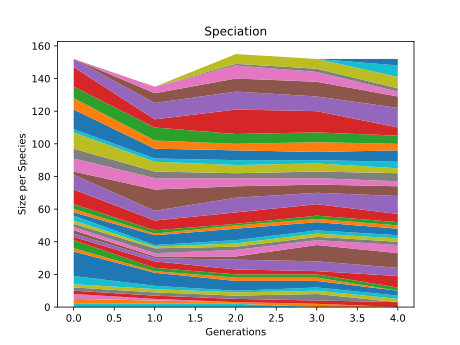
\includegraphics[width=.7\linewidth]{./speciation.png}
\caption{\label{fig:posvsfreq}
Speciation over generations
}
\end{figure}   
\begin{figure}[H]
\centering
\includegraphics[width=.7\linewidth]{./avg_fitness.png}
\caption{\label{fig:posvsfreq}
Evolution of fitness over generations
}
\end{figure}   
\label{sec:org70c3ecf}
\section{Conclusion}
\label{sec:org9f73321}
The results of this project are quite successful.
Although it is unable to complete other levels, it is able 
to complete level 1-1. However, random movements within the game, like the movement of enemies causes some inconsistencies
in the results.

An animated video containing an explanation and demonstration of the program can be found
at \url{https://youtu.be/JcxhGDdjCZ8}

\end{multicols}
\end{document}
